\documentclass[11pt,a4paper]{article}
\usepackage[utf8]{inputenc}
\usepackage[french]{babel}
\usepackage[T1]{fontenc}

\usepackage{amsmath}
\usepackage{amsfonts}
\usepackage{amssymb}

\newcommand{\NomAuteur}{Fabrice BOISSIER}
\newcommand{\TitreMatiere}{Système d'Exploitation}
\newcommand{\NomUniv}{EPITA - Bachelor Cyber Sécurité}
\newcommand{\NiveauUniv}{CYBER1}
\newcommand{\NumGroupe}{CYBER1}
\newcommand{\AnneeUniv}{2021-2022}
\newcommand{\DateExam}{18 février 2022}
\newcommand{\TypeExam}{Examen}
\newcommand{\TitreExam}{\TitreMatiere}
\newcommand{\DureeExam}{1h}
\newcommand{\MyWaterMark}{\AnneeUniv} % Watermark de protection

% Ajout de mes classes & definitions
\usepackage{MetalExam} % Appelle un .sty

% "Tableau" et pas "Table"
\addto\captionsfrench{\def\tablename{Tableau}}

%%%%%%%%%%%%%%%%%%%%%%%
%Header
%%%%%%%%%%%%%%%%%%%%%%%
\lhead{\TypeExam}							%Gauche Haut
\chead{\NomUniv}							%Centre Haut
\rhead{\NumGroupe}							%Droite Haut
\lfoot{\DateExam}							%Gauche Bas
\cfoot{\thepage{} / \pageref*{LastPage}}	%Centre Bas
\rfoot{\texttt{\TitreMatiere}}				%Droite Bas

%%%%%

\usepackage{tabularx}

\newlength{\LabelWidth}%
%\setlength{\LabelWidth}{1.3in}%
\setlength{\LabelWidth}{1cm}%
%\settowidth{\LabelWidth}{Employee E-mail:}%  Specify the widest text here.

% Optional first parameter here specifies the alignment of
% the text within the \makebox.  Default is [l] for left
% alignment. Other options are [r] and [c] for right and center
\newcommand*{\AdjustSize}[2][l]{\makebox[\LabelWidth][#1]{#2}}%


\definecolor{mGreen}{rgb}{0,0.6,0}
\definecolor{mGray}{rgb}{0.5,0.5,0.5}
\definecolor{mPurple}{rgb}{0.58,0,0.82}
\definecolor{backgroundColour}{rgb}{0.95,0.95,0.92}

\lstdefinestyle{CStyle}{
    backgroundcolor=\color{backgroundColour},
    commentstyle=\color{mGreen},
    keywordstyle=\color{magenta},
    numberstyle=\tiny\color{mGray},
    stringstyle=\color{mPurple},
    basicstyle=\footnotesize,
    breakatwhitespace=false,
    breaklines=true,
    captionpos=b,
    keepspaces=true,
    numbers=left,
    numbersep=5pt,
    showspaces=false,
    showstringspaces=false,
    showtabs=false,
    tabsize=2,
    language=C
}


\hyphenation{op-tical net-works SIGKILL}


\begin{document}

% \MakeExamTitleDuree     % Pour afficher la duree
\MakeExamTitle                   % Ne pas afficher la duree

%% \MakeStudentName    %% A reutiliser sur chaque nouvelle page

% Questions cours Apache/HTTP
\section{Systèmes de fichiers (8 points)}

%\begin{figure}[ht!]
%\centering
%\centerline{
%\includegraphics[scale=1]{images/ModeleWI.png}
%}
%\caption{Modele d'image}
%\label{figure:1-S1-ModeleWI}
%\end{figure}

\begin{figure}[ht!]
\centering
\centerline{
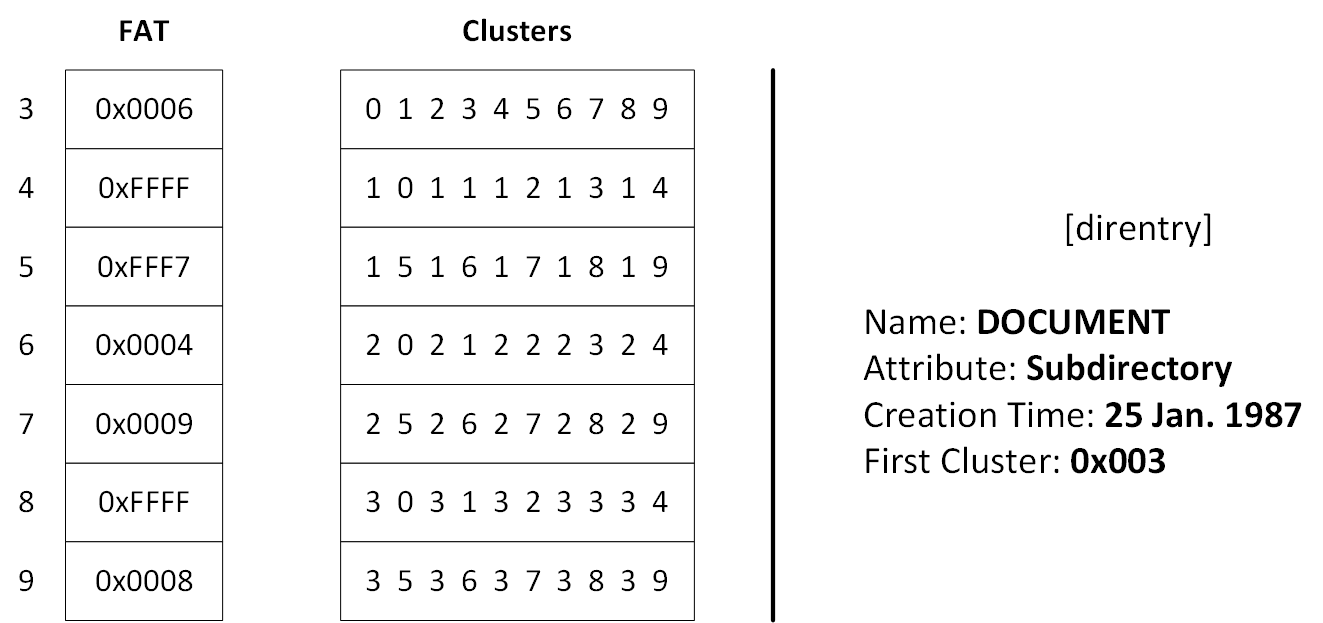
\includegraphics[scale=1]{FAT1-Direntry.png}
}
%\caption{Modele d'image}
%\label{figure:1-S1-ModeleWI}
\end{figure}


\subsection{(1 point) Quelle séquence de chiffres correspond à \og DOCUMENT \fg ? }

\bigskip

%\TextField[comb,maxlen=3,name=accountA,width=3em]{}
%\TextField[comb,maxlen=3,name=accountA,width=3em,bordercolor=]{}
%\TextField[comb,name=reponse1,charsize=18pt,maxlen=10,width=20em,height=0.8cm,bordercolor=black,backgroundcolor=white,bordersep=10pt]{\AdjustSize[l]{label}}

\centerline{
\TextField[comb,
name=reponse1,
charsize=18pt,
maxlen=30,
width=19cm,
height=1cm,
bordercolor=black,
backgroundcolor=white,
bordersep=10pt[]{}
%default=012345678920212223241011121314]{}
%value=012345678920212223241011121314]{}
}

\bigskip

\subsection{(1 point) En admettant qu'un \underline{fichier} est stocké dans cette FAT (en plus de \og DOCUMENT \fg), à quel cluster semble-t-il démarrer ?}

\bigskip
\bigskip  % Cluster 5
\bigskip

\subsection{(0,5 point) En admettant que les clusters et secteurs font 4.096 octets, et que la \textit{direntry} du fichier indique en size 11.042 octets. Combien d'octets faut-il ignorer dans le dernier cluster ?}

\bigskip
\bigskip  % 4.096 * 3 = 12.288
\bigskip  % 12.288 - 11.042 = 1.246
\bigskip

\subsection{(1 point) Un fichier contenant 10.000 caractères est stocké sur un système de fichiers dont les clusters font 4.096 octets et les secteurs font 512 octets. Quelle taille en octets consomme-t-il sur le support physique et combien de secteurs consomme-t-il ?}

\bigskip
\bigskip
\bigskip  %  8192 octets et 16 secteurs
\bigskip


\newpage

\subsection{(2 points) Dans quelle situation ou action peut-on se rendre compte qu'une telle FAT ne fonctionne pas/n'est pas viable pour stocker des données ? (selon les règles que vous avez apprises) Et pourquoi n'est-elle pas viable ?}

\bigskip

\begin{figure}[ht!]
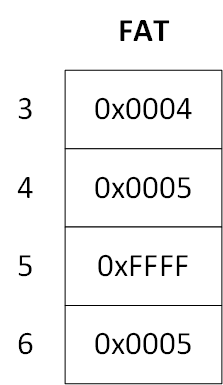
\includegraphics[scale=1,left]{FAT2.png}
%\caption{Modele d'image}
%\label{figure:1-S1-ModeleWI}
\end{figure}

\bigskip  % Lors de la suppression, on devra éliminer la fin d'un autre fichier.

\subsection{(1 point) En quoi les \textit{i-nodes} et \textit{direntry} d'ext2 sont-ils différents ?}

\bigskip
\bigskip
\bigskip  % L'inode contient les propriétés de chaque ressource ainsi que la liste des blocs contenant la ressource.
\bigskip  % Les direntry contiennent juste une liste de ressources dans un dossier et quel inode les décrit.
\bigskip
\bigskip

\subsection{(0,5 point) Dans quelle(s) structure(s) trouve-t-on le nom des fichiers ?}

\bigskip
\bigskip  % Dans les direntry
\bigskip

\subsection{(1 point) Expliquer la différence entre \og \textit{hardlink} \fg et \og \textit{symbolic link} \fg.}

\bigskip
\bigskip  % Hardlink : une direntry contient une entrée typée "hardlink" qui pointe vers l'inode de la ressource
\bigskip  % Symlink : c'est un inode dont les blocs contiennent le chemin vers la ressource visée (qui a son propre inode)
\bigskip
\bigskip
\bigskip


%
\section{Ordonnancement et Processus (4 points)}

\subsection{(1 point) Citer les états dans lesquels un processus peut se trouver.}

\bigskip
\bigskip  % Execution/Running, Asleep, Ready
\bigskip

\subsection{(1 point) Expliquez succinctement pourquoi on ne peut pas tuer avec SIGKILL un processus en état "Zombie".}

\bigskip
\bigskip  % SIGKILL retire un processus de l'ordonnanceur, mais il ne supprime pas le PCB/la structure permettant au
\bigskip  %  processus parent d'être informé de la mort de son fils.
\bigskip
\bigskip

\newpage

\subsection{(2 point) Dessinez la hiérarchie de processus créée par ce programme C :}

%\bigskip
%\begin{lstlisting}[style=CStyle]
%int main(void)
%{
%  pid_t p1, p2, p3;
%
%  p1 = fork();
%  if (p1 > 0) {
%    // Process A
%    p2 = fork();
%    if (p2 > 0) {
%      // Process B
%    } else { // Process C }
%  } else {
%    //Process D
%    p3 = fork();
%    if (p3 > 0) {
%      // Process E
%    } else { // Process F }
%  }
%}
%\end{lstlisting}
%\bigskip

\noindent\begin{minipage}{.45\textwidth}
\begin{lstlisting}[style=CStyle]
int main(void)
{
  pid_t p1, p2, p3;

  p1 = fork();
  if (p1 > 0) {
    // Process A
    p2 = fork();
    if (p2 > 0) {
      // Process B
    } else { // Process C }
  } else {
    //Process D
    p3 = fork();
    if (p3 > 0) {
      // Process E
    } else { // Process F }
  }
}
\end{lstlisting}
\end{minipage}\hfill
\begin{minipage}{.45\textwidth}
\begin{lstlisting}[showlines=true,backgroundcolor=\color{white},numbersep=5pt,showspaces=false,showstringspaces=false,showtabs=false,tabsize=2]















\end{lstlisting}
\end{minipage}


%
\section{Script Shell et Commandes (8 points)}

\subsection{(3 points) Expliquez ce que font ces lignes de commandes :}

\bigskip

%\TTBF{ps aux | sort -k 2,2n | tail -n 10 > file1.txt }
\TTBF{ps aux | head -n 20 | tail -n 10 > file1.txt }

\bigskip

\LigneReponseCinq

\bigskip


%\TTBF{cat /etc/passwd | cut -d ":" -f 1 | grep "metalman" > file2.txt}
\TTBF{touch file3.txt \&\& cat /etc/passwd | grep "metalman" > file2.txt}

\bigskip

\LigneReponseCinq

\bigskip


\TTBF{cat file1.txt < file2.txt 1> file3.txt 2> file4.txt}

\bigskip

\LigneReponseCinq

%\bigskip

\newpage

\subsection{(5 point) Indiquez à quoi sert chaque opérateur, et donnez un exemple.}

% Allonge les cases en hauteur
\renewcommand\arraystretch{1.5}

%\bigskip

\begin{center}
%  \begin{tabularx}{11cm}{| c | p{2cm} | p{2cm} |}
  \begin{tabularx}{18cm}{| c | *{1}{>{\centering \arraybackslash}X |}} % \linewidth
  \hline
  Opérateur & Exemple et explication \\ \hline
   & \\
   & \\
   & \\
  \TTBF{>} & \\
   & \\
   & \\
   & \\
   \hline
   & \\
   & \\
   & \\
  \TTBF{>{}>} & \\
   & \\
   & \\
   & \\
   \hline
   & \\
   & \\
   & \\
  \TTBF{<} &  \\
   & \\
   & \\
   & \\
   \hline
   & \\
   & \\
   & \\
  \TTBF{<{}<} & \\
   & \\
   & \\
   & \\
   \hline
   & \\
   & \\
  \TTBF{|} & \\
   & \\
   & \\
   \hline
  \end{tabularx}
\end{center}
\medskip

\renewcommand\arraystretch{1}

\newpage


\end{document}
